\chapter{Теорія функціоналу густини}
Переважна теоретична картина твердотільних та / або молекулярних систем включає неоднорідний електронний газ: набір взаємодіючих точкових електронів, що рухаються квантово-механічно в потенційному полі набору атомів, які вважаються статичними (наближення Борна–Оппенгеймера). Рішення таких моделей зазвичай вимагає використання схем апроксимації, з яких найбільш основною являється апроксимація незалежних електронів, теорія Хартрі і теорія Хартрі–Фока — зазвичай викладаються студентам на курсах фізики і хімії. Однак існує інший підхід - теорія функціоналу густини (ТФГ), яка за останні тридцять років або близько того все частіше стає методом який обирають для вирішення завдань розрахунку багаточастинкових систем. Цей метод має подвійну перевагу: він дозволяє вирішувати багато завдань з досить високою точністю, а також є простим в обчислювальному відношенні (простіше навіть, ніж схема Хартрі). Незважаючи на ці переваги, він відсутній у більшості програм бакалаврату та багатьох програм магістратури, з якими ми знайомі.
\section{Загальна теорія}
У цьому розділі представлено єдине трактування термодинаміки і теорії функціоналу густини. Для простоти спочатку буде розглянуто випадок класичної взаємодіючої системи частинок. Читачеві рекомендується мати на увазі електронні системи, які будуть предметом наступного розділу. Таким чином, рів. \ref{eqn:Ham_}--\ref{eqn:free_energ_functional}, які будуть виведені тут з використанням класичних позначень, в рівній мірі застосовні до квантово-механічних систем, де гільбертовий простір з його операторами положення і імпульсу замінює класичний фазовий простір і його скалярні координати.
\subsection{Термодинаміка}
Ми розпочнемо з переосмислення рівнянь термодинаміки в застосунку до квантовомеханічних систем. Спочатку розглянемо класичну систему з N взаємодіючих частинок в об'ємі V. Гамільтоніан такої системи буде наступним:
\begin{equation}
\label{eqn:Ham_}
	{\cal H}_{mb} = {\cal T} + {\cal U},
\end{equation}
де ${\cal T} = \sum\limits_{i}\textbf{p}_i^2/2m$ -- кінетична енергія $i$-тої частинки та ${\cal U} = \sum_{i < j}u(|\textbf{r}_i - \textbf{r}_j|)$ -- енергія взаємодії у вигляді простого парного потенціалу $u(r)$. Тут $\textbf{p}_i$ та $\textbf{r}_i$ -- координата та імпульс у просторі, $m$ -- її маса. 
Ми розглянемо великий канонічний ансамбль, де система знаходиться у контакті з джерелом тепла з температурою $T$ і з частинковим резервуаром з хімічним потенціалом $\mu$. Як вже відомо з статистичної фізики потенціал вільної енергії у даному випадку задається наступним чином:

\begin{equation}
\label{eqn:omegapotential}
	\Omega(\mu,T,V) = -T\log\Xi,
\end{equation}
 
де $\Xi$ функція омега-розподілу:

\begin{equation}
\label{eqn:sgranddistr}
	\Xi(\mu, T, V) = \sum\limits_{M = 0}^\infty\frac{1}{M!}Tr\exp{\left(-\frac{{\cal H}_{mb} - {\mu} M}{T}\right)},
\end{equation}

температура вказана в одиницях енергії (тобто $k_{B} = 1$), а класичний слід, $Tr$, представляє $6M$-мірний інтеграл по фазовому простору (поділ на $M!$ компенсує подвійний підрахунок станів багатьох тіл нерозрізнених частинок). 

З цих визначень безпосередньо випливає, що математичне очікування числа частинок в системі задається похідною від омега-потенціалу, $N = \langle M \rangle = -(\partial{\Omega}/\partial{\mu})$. Опуклість термодинамічного потенціалу \cite{convexfreeenerg} дає, що $N$ являється функцією $\mu$. Інші часткові похідні $\Omega$ дають значення додаткових фізичних величин, таких як ентропія $S$ та тиск $P$ це може бути узагальнено таким чином $d\Omega = -Nd\mu - SdT - PdV$

В різних контекстах ми повинні використовувати різні ансамблі. Наприклад, при досліджені системи в якій кількість частинок постійна, а хімічний потенціал ні, то краще використовувати вільну енергію Геймгольца, яку можна отримати з омега-потенціалу $\Omega$ за допомогою перетворення Лежандра: $F(N,T,V) = \Omega(\mu(N),T,V)+\mu(N)N.$
Тут $\mu(N)$ більше не являється незалежною змінною, але функція N отримується за допомогою інвертування співвідношення $N = N({\mu},T,V)=\dfrac{\partial\Omega}{\partial\mu}.$ Похідна $F$ по відношенню до "нової" \ вільної змінної $N$ дорівнює до "старої" \ змінної $\mu$. Інші похідні не змінюються. Тому ми можемо записати наступне $dF={\mu}dN - SdT - PdV$.

Для порівняння з DFT буде корисно зробити варіацію оберненого перетворення Лежандра, яке виражає потенційну енергію $\Omega$ у термінах вільної енергії $F$ і визначимо наступний омега-потенціал, як функцію, яка залежить явно від $\mu$ та $N$:
\begin{equation}
	\label{eqn:grand-potentialfunc}
	\Omega_\mu \equiv F(N,T,V) - {\mu} N
\end{equation}
Ця функія дає початковий омега-потенціал рівняння \ref{eqn:omegapotential} при мінімізації відносно $N$, тобто коли похідна $(\partial{F}/\partial{N}) - \mu$ зникає, що еквівалентно умові $N = N(\mu,T,V)$ за звичаї, яке використовується у оберненому перетворені Лежандра. Для геометричної інтерпретації перетворення Лежандра дивіться рис. \ref{fig:legander_transform}
\begin{figure}[H]
  \centering
  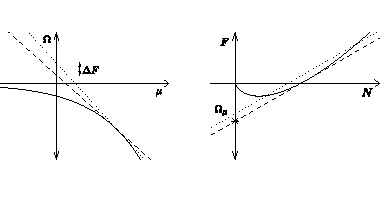
\includegraphics[scale=2.5]{img/Legender_transform.pdf}
  \caption{(a) Перетворення Лежандра, яке дає $F(N)$, відповідає опису кривої $\Omega\mu$ властивостями її дотичних: мінус їх нахили $N = -(\partial{\Omega}/\partial{\mu})$. та їх перетину з енергетичною віссю, $F = \Omega + \mu N$. Той факт, що похідна $\Delta F / \Delta N$ дорівнює $\mu$, слідує з формулювання питання: якщо дві сусідні прямі перетинають енергетичну вісь на відстані $\Delta F$ один від одного і мають нахили, які відрізняються на $\Delta N$, на якій відстані від осі вони будуть перетинати один одного? (b) Зворотне перетворення Лежандра з $F(N)$ в $\Omega (\mu)$ має аналогічну інтерпретацію. Мінімізація, запропонована в рівнянні. \ref{eqn:grand-potentialfunc} відповідає вивченню сімейства ліній з фіксованим нахилом $\mu$, які проходять через точки $N, F$ на кривій вільної енергії. Їх перетин, має мінімум (зазначений зірочкою) для тієї лінії, яка є дотичною до кривої \cite{Argaman_2000}.}
  \label{fig:legander_transform}
\end{figure}
\subsection{Підхід Кона-Шема}
Наведене вище обговорення можна досить просто узагальнити на обробку частинок у зовнішньому потенціалі $v(\textbf{r})$. Гамільтоніан багатьох тіл тепер дорівнює
\begin{equation}
\label{eqn:Ham}
	{\cal H}_{mb} = {\cal T} +{\cal V} +{\cal U},
\end{equation}
де ${\cal V} = \sum\limits_{i=0}^M v(\textbf{r}_i)$ -- потенційна енергія. Омега-потенціал і омега-функція були визначені як рів.\ref{eqn:omegapotential} та \ref{eqn:grand-potentialfunc}, але зараз вони залежать від потенціальної функції $v(\textbf{r})$, а не скалярного об'єму $V$. Тому $\Omega = \Omega(\mu, T, [v(\textbf{r})])$ тепер є функціоналом $v(\textbf{r})$, а тако ж функцією $\mu$ і $T$ -- квадратні дужки позначають функціональні змінні. 

Як добре відомо, потенціал $v(\textbf{r})$ - це енергія, яка вимірюється з довільного джерела, тобто Зміщення потенціалу на постійну величину не впливає на фізику системи. Тут зручно встановити цей початок координат в хімічному потенціалі, тобто прийняти $\mu = 0$. Еквівалентно, можна визначити нову функціональну змінну як $v(\textbf{r}) - \mu$, оскільки $\Omega$ залежить тільки від цієї різниці, а не від $v(\textbf{r})$ і $\mu$ окремо.

Функціональна похідна $\Omega$ за новою змінною дає розподіл щільності частинок, $n(\textbf{r}) = \langle \rho (\textbf{r}) \rangle$, де $\rho(\textbf{r}) = \sum\limits_{i=1}^M\delta(\textbf{r}-\textbf{r}_i)$ неперевірена щільність. Використовуючи (функціональне) перетворення Лежандра, як зазначено вище, ми можемо визначити нову вільну енергію, яка залежить від $n(\textbf{r})$, а не від $v(\textbf{r})$, і називається вільною енергією Хоенберга-Кона:
\begin{equation}
	\label{eqn:free_energ_hoenberg-khon}
	F_{HK}[n(\textbf{r})] = \Omega[v(\textbf{r})] - \int{n(\textbf{r}) v(\textbf{r})d\textbf{r}} 
\end{equation}
де зміною температури у явному вигляді ми знехтували і $v(\textbf{r)}$ з правої частини обрана так, щоб відповідати заданому $n(\textbf{r})$ (такий вибір можливий лише із-за загальної опуклості вільної енергії). Частина та функціональна похідна $F_{HK}[n(\textbf{r})]$ задається звичайним правилом перетворення Лежандра, як: $dF_{HK} = -SdT - \int{v(\textbf{r})\delta n(\textbf{r})d\textbf{r}}$.
Пряме узагальнення функції вильної енергії це і є функціонал вільної енергії:
\begin{equation}
	\label{eqn:free_energ_functional}
	\Omega[n(\textbf{r})] \equiv F_{HK}[n(\textbf{r})] + \int{n(\textbf{r})v(\textbf{r})d\textbf{r}}
\end{equation}
Якщо цей функціонал мінімізувати відносно $n(\textbf{r})$ і при постійному $v(\textbf{r})$ то функціонал вільної енергії дорівнює омега-потенціалу. Існування функціоналу $n(\textbf{r})$ з цією властивістю є одним з основних принципів DFT і є другою теоремою Хоенберга–Кона (див. наступний параграф).

Обговорення теореми Хоенберга-Кона, тим не менш, важливо навіть у введенні до DFT на основі перетворення Лежандра, оскільки процедура мінімізації вільної енергії, втілена в ньому, є центральною як для формування фізичної інтуїтивної картини DFT, так і для розробки ефективних чисельних схем для вирішення рівнянь DFT в практиці.

Узагальнюючи можна сказати, що в DFT Кона-Шема всі обмінні та кореляційні ефекти включені в обмінно-кореляційний функціонал $E_{xc}[n]$, котрий залежить від густини $n(\textbf{r})$ електронів. 


Функціонал повної енергії може бути записаний, як \cite{KSenergy}:
\begin{eqnarray}
 E[\psi_i] = 2\sum\limits_{i}\int\psi_i\left({{\hbar^2}\over{2m}}\right)\nabla^2\psi_id^3\textbf{r}+\int V_{ion}(\textbf{r})n(\textbf{r})d^3\textbf{r}+\nonumber \\
 {{e^2}\over{2}}\int {{n(\textbf{r})n(\textbf{r})}\over{|\textbf{r}-\textbf{r}^\prime|}}d^3\textbf{r}d^3\textbf{r}^\prime+E_{xc}[n(\textbf{r}^\prime)]+E_{ion}(R_i)
\end{eqnarray}

Де $V_{ion}$ -- повний електрон-іонний потенціал, $E_{xc}[n(\textbf{r}^\prime)]$ -- обмінно-кореляційний функціонал, $E_{ion}$ -- кулонівська енергія, $n(\textbf{r})$ -- електронна густина

\section{Теореми Кона-Шема}
Шляхом публікації двох статей Хохенбергом та Коном у 1964 році~\cite{Hohenberg&Khon}, а також Коном і Шемом в 1965 році~\cite{Khon&Sham}, в яких доводились теореми завдяки яким теорія функціоналу ґустини вийшла на новий рівень. Ці теореми встановлюють точну відповідність між електронною щільністю, зовнішнім потенціалом і хвильовою функцією.

\textbf{Перша теорема} говорить про те, що електронна щільність єдиним чином визначає оператор Гамільтона і, отже, всі характеристики системи.
Не можуть існувати два різні зовнішні потенціали, що призводять до однієї і тієї ж електронної щільності основного стану системи, іншими словами, електронна щільність основного стану однозначно визначається зовнішнім потенціалом.
Знаючи потенціал, ми знаємо Гамільтоніан системи, відповідно можемо знайти хвильову функцію системи та всі властивості системи, що визначаються електронною щільністю основного стану. Перша теорема показує зв'язок між зовнішнім потенціалом та електронною щільністю основного стану.

\textbf{Друга теорема} функціонал енергії, що визначає енергію квантового стану системи, визначає мінімальну енергію тоді і тільки тоді, коли електронна густина, що входить у функціонал, є реальною густиною основного квантового стану.
Таким чином, для знаходження точної енергії основного стану та його щільності, достатньо знати функціонал $E[n]$. Висновки цих теорем призводять до того, що для будь-якого зовнішнього потенціалу завжди можна знайти електронну густину та енергію основного стану, мінімізуючи цей функціонал.


\subsection{Самоузгоджене рівняння Кона-Шема}
Електронна щільність системи може бути знайдена з рішення самоузгодженого рівняння Кона-Шема, це випливає з наведених раніше теорем, яке можна записати так:

\begin{equation}
    \left[{{-\hbar^2}\over{2m}}\nabla^2+V_{ion}(\textbf{r})+V_H(\textbf{r})+V_{XC}(\textbf{r})\right]\psi_i(\textbf{r}) = e_i\psi_i(\textbf{r})
\end{equation}

Де $\psi_i$ -- хвильова функція стану $i$, $e_i$ -- власні значення, $V_H$ -- потенціал Хартирі, який відповідає за електронно-електронне відштовхування.

Явний вид обмінно-кореляційного потенціалу $V_{XC}$ ми не можемо знати принципово, тому його задають формально, функціональною похідною: 

\begin{equation}
    V_{XC} = \frac{\partial E_{XC}[n(\textbf{r})]}{\partial n(\textbf{r})}
\end{equation}

Для визначення об'ємно-кореляційного потенціалу використовують ряд наближень, про які ми поговоримо у наступному розділі.


\section{Методи апроксимації \textbf{$E_{xc}$}}
\subsection{LDA}
LDA (local density approximation) -- це клас наближень для обмінно-кореляційної енергії $E_{XC}$ у DFT, яка залежить виключно від електронної густини в кожній точці простору. Найуспішнішими локальними наближеннями є ті, що були отримані з моделі однорідного електронного газу (HEG)~\cite{Hohenberg&Khon}. 

Можна записати наступний вираз для обмінно-кореляційної енергії:

\begin{equation}
    E_{XC}^{LDA}[n(\textbf{r})] = \int{\epsilon_{xc}[n(\textbf{r})]n(\textbf{r})d^3\textbf{r}}
\end{equation}

Існує ряд параметрів для LDA, але ми їх не розглядатимемо.

\subsection{GGA}
GGA (generalized gradient approximations) -- на відміну від LDA в даний клас наближень включено градієнтну поправку для електронної щільності. Це усуває деякі недоліки LDA. Для узагальненого градієнтного наближення ми можемо записати, що $E_{xc}$ дорівнює деякій функції локальної щільності та її градієнта:

\begin{equation}
    E_{xc}^{GGA} = \int{\epsilon_{xc}[n(\textbf{r}),\nabla{n(\textbf{r})]n(\textbf{r})d^3\textbf{r}}}
\end{equation}

Найчастіше для розрахунків використовуються параметризації PBE (Perdew-Burke-Ernzerhof)~\cite{PBE} та PW91~\cite{PW91}.

\subsection{meta-GGA}
Фактично meta-GGA - це розширене наближення GGA. В яке, як вхідні дані, входить щільність позитивної орбітальної кінетичної енергії~\cite{Swapan&Gosh&Parr, Becke&Roussel, Tao&Perdew}.

У напівлокальному наближенні функціонал $E_{xc}$ зводиться до єдиного інтегралу загального вигляду:
\begin{equation}
    E_{XC}^{MGGA} = \int{\epsilon_{xc}[n(\textbf{r}),\nabla{n(\textbf{r}),\tau_{\sigma}(\textbf{r}})]}n(\textbf{r})d^3\textbf{r}
\end{equation}

Де $\tau_{\sigma}(\textbf{r})$ щільність кінетичної енергії зайнятих станів та визначається як:
\begin{equation}
    \tau_{\sigma}(\textbf{r}) = \sum\limits_{i\textbf{k}}|\nabla\psi_{i\textbf{k}}(\textbf{r})|^2
\end{equation}
\subsubsection{SCAN}
SCAN (Strongly-constrained and appropriately-normed) meta-GGA, раніше розроблені meta-GGA функціонали виявилися менш точними для розрахунку критичних тисків у структурно-фазових переходах твердих тіл, а також для матеріалів з шаруватою структурою відомі, як Ван-дер-Ваальсовські матеріали. SCAN покликаний усунути цю проблему за допомогою додавання в обмінно-кореляційний функціонал безрозмірну змінну.
$\alpha$~\cite{SCAN}:
\begin{equation}
    \alpha = (\tau - \tau^W)/\tau^{unif} > 0
    \label{eqn:alpha}
\end{equation}

Де $\tau^W = |\nabla{n(\textbf{r})}|^2/8n(\textbf{r})$ є одноорбітальною межею $\tau$ \newline та $\tau^{unif} = (3/10)(3\pi^2)^{2/3}n(\textbf{r})^{5/3}$ межа рівномірної щільності.

Відомо багато особливостей точного функціоналу $E_{xc}$. неемпіричні функціонали, побудовані для задоволення точних обмежень на цей функціонал щільності, надійні в широкому діапазоні систем (наприклад, атомів, молекул, твердих тіл і поверхонь), включаючи багато, які не схожі на ті, для яких ці функціонали були протестовані і підтверджені. У цьому розділі ми більш глибше розкриємо імплементацію функціоналу, який вперше задовольняє всім відомим можливим точним обмеженням \hyperref[lst:Constrains]{[Список 2.1]} і відповідним чином нормується в системах, для яких напівлокальні функціонали можуть бути точними або надзвичайно точними.

\begin{itemize}	
\label{lst:Constrains}
   \item Для обмінної енергії
   \begin{itemize}
     \item Негативність 
     \item Спінове масштабування
     \item Однорідне масштабування щільності
     \item Неоднорідне масштабування щільності
     \item Розширення градієнту четвертого порядку
     \item Жорстка межа для двохелектронних щільностей
   \end{itemize}
   \item Для кореляційної енергії
   \begin{itemize}
   	  \item Негативність
   	  \item Розширення градієнту другого порядку
   	  \item Рівномірне масштабування щільності до межі високої щільності
   	  \item Рівномірне масштабування щільності до межі низької щільності
   	  \item Нульова енергія кореляції для будь-якої одноелектронної спін-поляризованої щільності
   	  \item Нерівномірне масштабування щільності
   	  \item Масштабуємітсь розмірів системи
   	  \item Границя Ліба-Оксфорда
   	  \item Слабка залежність від відносної спінової поляризації в межі низької щільності
   	  \item Статичний лінійний відгук однорідного електронного газу
   	  \item Межа Ліба-Оксфорда для двох густин електронів
   	\end{itemize}
 \captionof{constrains}{Обмеження для обмінно-кореляційної енергії $E_{xc}$.}
 \end{itemize}

Запишемо кореляційну енергію $\epsilon_c$ на один електрон рів. \ref{eqn:e_c}. Також намалюємо фактор посилення \ $F_{xc}(r_s, \xi, s, a)$ в наближені низької густини $r_s \rightarrow \infty$ \ref{fig:F_factor}. Тут $\xi = (n_\uparrow - n_\downarrow)/(n_\uparrow + n_\downarrow)$ спін поляризація, $r_s = (4 \pi n/3)^{-1/3}$, і $s = {|\nabla{n}|}/{2(3\pi^2)^{-1/3}
\\ n^{4/3}}$, $\alpha$ -- безрозмірний параметр \ref{eqn:alpha}. 

Напівлокальний обмінно-кореляційний функціонал можна записати наступним чином (знехтуємо $\nabla \xi$ та припустимо що параметр $\alpha$ однаковий для спін-неполяризаційних густин $2n_\uparrow$ та $2n_\downarrow$):

\begin{equation}
	\label{eqn:semilocalexc}
	E_{xc}[n_{\uparrow},n_{\downarrow}] = \int{d^3 r n\epsilon_{xc} = \int d^3 r n \epsilon_{x}(n)F(r_s,\xi, s, a)}
\end{equation}

Де $\epsilon_x^{unif} = -(3/4\pi)(3\pi^2n)^{1/3}$ обмінна енергія на електрон однорідного електронного газу.  
Кореляційну частину можна записати як: 

\begin{equation}
	\label{eqn:cor}
	E_{c}[n_{\uparrow},n_{\downarrow}] = \int{d^3 n \epsilon_c (r_s,\xi, s, a)}
\end{equation}

SCAN $\epsilon_c$ має наступну форму:

\begin{equation}
	\label{eqn:e_c}
	\epsilon_c = \epsilon_c^1 + f_c(\alpha)(\epsilon_c^0 -\epsilon_c^1)
\end{equation}

Де $f_c(a) = exp[-c_{1c}\alpha/(1-\alpha)]\theta(1-\alpha)-d_c exp[c_{2c}/(1-\alpha)]\theta(\alpha-1)$

У статі \cite{SCAN} переглядають форму PBE функціоналу для більш точного підходу до 2D межі при нерівномірному масштабуванні: 
\begin{equation}
	\epsilon_c^1 = \epsilon_c^{LSDA1}+H_1
\end{equation}

Де

\begin{equation}
	\label{eqn:H_1}
	H_1 = \gamma\phi^3ln[1+w_1(1-g(At^2))],
\end{equation}

\begin{equation}
	t = (3\pi^2/16)^{1/3}s/(\phi r_s^{1/2}),
\end{equation}

\begin{equation}
	w_1 = exp[-e_c^{LSDA1}/(\gamma\phi^3)] - 1,
\end{equation}

\begin{equation}
	A = \beta(r_s)/(\gamma w_1),
\end{equation}

\begin{equation}
	g(At^2) = 1 / (1 + 4At^2)^{1/4}.
\end{equation}

$\epsilon_c^{LSDA1}$ кореляційна енергія однорідного електронного газу. Тут використовується PW92 LSDA параметризація \cite{PhysRevB.45}. Де $\gamma = 0.0391091$, $\beta(r_s) = 0.066725(1 + 0.1r_s)/(1 + 0.1778r_s)$ \cite{PhysRevLett.103}, та $\phi = [(1 + \xi)^{2/3} + (1 - \xi)^{2/3}]/2$. $\epsilon_c^1$ відрізняється від оригінальної PBE кореляції тільки в виразах для $\beta(r_s)$ та $g(At^2)$. Оригінальна кореляційна енергія з PBE  функціоналу \cite{PBE} має для цих виразів наступні значення $\beta(r_s) = 0.066725$ та $g(At^2) = 1 / (1 + At^2 + A^2 t^4)$.

Таким чином можна надати вигляд $\epsilon_c^0$ за аналогією до $\epsilon_c^1$, реалізація цього відбувається за умови, що для $\alpha = 0$ може виникнути зміна градієнту густини s:
\begin{equation}
	\epsilon_c^0 = (e_c^{LDA0} + H_0) G_c(\xi),
\end{equation}

Де 

\begin{equation}
	\label{eqn:G_c}
	G_c(\xi) = \big\{1 - 2.3631[d_x(\xi) - 1]\big\} (1 - \xi^12), 
\end{equation}

\begin{equation}
	d_x(\xi) = [(1+\xi)^{4/3} + (1 - \xi)^4/3] / 2,
\end{equation}

\begin{equation}
	\epsilon_c^{LDA0} = -b_{1c}/(1+b_{2c}r_s^{1/2}+b_{3c}r_s)
\end{equation}

Вираз $G_c(\xi)$ \ref{eqn:G_c} був спроєктований щоб кореляційна енергія зверталася в нуль для будь-якої електронної щільності та зробити $F_{xc}(r_s \rightarrow \infty, \xi, s = 0, \alpha = 0)$ незалежним від $\xi$ для $0 \leq |\xi| < 0.7$. Точна обміно-кореляційна енергія в межі низької щільності не залежить від $\xi$. Це здобувається за допомогою s = 0 точно у $\alpha = 0$ і як можна краще у $\alpha = 0$. 

Аналогічно до $H_1$ \ref{eqn:H_1}, 

\begin{equation}
	H_0 = b_{1c}ln[1+w_0(1 - g_\infty(\xi = 0, s))], 
\end{equation} 

Де 
\begin{equation}
	w_0 = exp[-e_c^{LDA0}/b_{1c}]-1,
\end{equation}
\begin{equation}
	g_\infty(\xi,s) = \lim_{r_s \rightarrow \infty}g(At^2) = 1 / (1 + 4\chi_\infty s^2)^{1/4}.
\end{equation}
Де $\chi_\infty(\xi) = \left(\frac{3\pi^2}{16}\right)^{\frac{2}{3}}\beta(r_s \rightarrow \infty)\phi/[c_x(\xi)-f_0]$, $c_x(\xi) = -(3/4\pi)(9\pi/4)^{1/3}d_x(\xi)$, $f_0 = -0.9$. При $\xi = 0$, $ \chi_\infty(\xi = 0) = 0.128026$.

Параметри $b_{1c} = 0.0285764$, $b_{2c} = 0.0889$, $b_{3c} = 0.125541$, визначаються у наступній процедурі:

У межі великої густини, $e_c^0 = b_{1c}G_c(\xi)ln\{1 - g_\infty(\xi = 0, s)exp(1)/[exp(1)+1]\}$ та $b_{1c} = 0.0285764$ за допомогою підгонки до кореляційної енергії $E_c = -0.0467 Ha$ високої густини двохелектронного іону з атомним номером $Z \rightarrow \infty$. $b_{3c} = 0.125541$ визначається нижчою межею обмінно-кореляційних енергій двохелектронної системи, $F_{xc} \leq 1.67082$. $b_{2c} = 0.0889$ підганяється до $E_{xc}(He) = -1.068 Ha$. Параметри у інтерполяційної/екстраполяційної функції наступні $c_{1c} = 0.64, c_{2c} = 1.5, d_c = 0.7$.

Сім параметрів ($c_{1x}, c_{2x}, d_x, k_1, c_{1c}, c_{2c}, d_c$) можна визначити наступним чином: для заданого $k_1$, ми підганяємо до 
\begin{enumerate}
    \item $\gamma_{x1} = -0.2259$, $\gamma_{x2} = 0.2551$, $\gamma_{c1} = 0.0388$ асимптотичні коефіцієнти великого Z для обміну і кореляції атомів рідкісних газів з атомним номером Z,
    \item Крива енергії зв'язку стисненого Ar$_2$ (із середньою абсолютною похибкою менше 1 ккал / моль для довжин зв'язків R=1.6, та 2.0 $\angstrom$),
    \item обмінно-кореляційна енергія поверхні желе при параметрі насипної щільності $r_s = 4 \ Bohr$ в межах 5\% від значення QMC \cite{PhysRevB.76}.
\end{enumerate}

Потім обирається набір параметрів з максимальним значенням $k_1$, оскільки точні енергії обміну для модельних густин металів з посилання \cite{PhysRevB.54} припускають, що $k_1$ не повинен бути занадто маленьким.

Для повноти, нарешті, можна навести розкладання градієнта четвертого порядку для енергії обміну, яке діє у наступному інтервалі $0 \leq s \ll 1$ та $a \approx 1:$

\begin{eqnarray}
	F_x^{GE4}(s,a) = 1+(10/81)s^2 - (1606/18225)s^4 +\nonumber \\
 + (511/13500)s^2(1-\alpha) + (5913/405000)(1-\alpha)^2.      
\end{eqnarray}

SCAN дуже добре пророкує певні властивості зв'язку: енергію атомізації, енергії зв'язку при слабкій взаємодії і константи решітки твердих тіл, але не енергетичні бар'єри для хімічних реакцій. Ми припускаємо, що перші три властивості природним чином потрапляють в область хорошого напівлокального функціоналу, в той час як четверте вимагає повністю нелокальної апроксимації (наприклад, корекція самовзоємодії для SCAN).
 
\begin{figure}[H]
\centering
\label{fig:F_factor}
	\begin{subfigure}{.9\textwidth}
		\hspace*{-1.2cm}
    	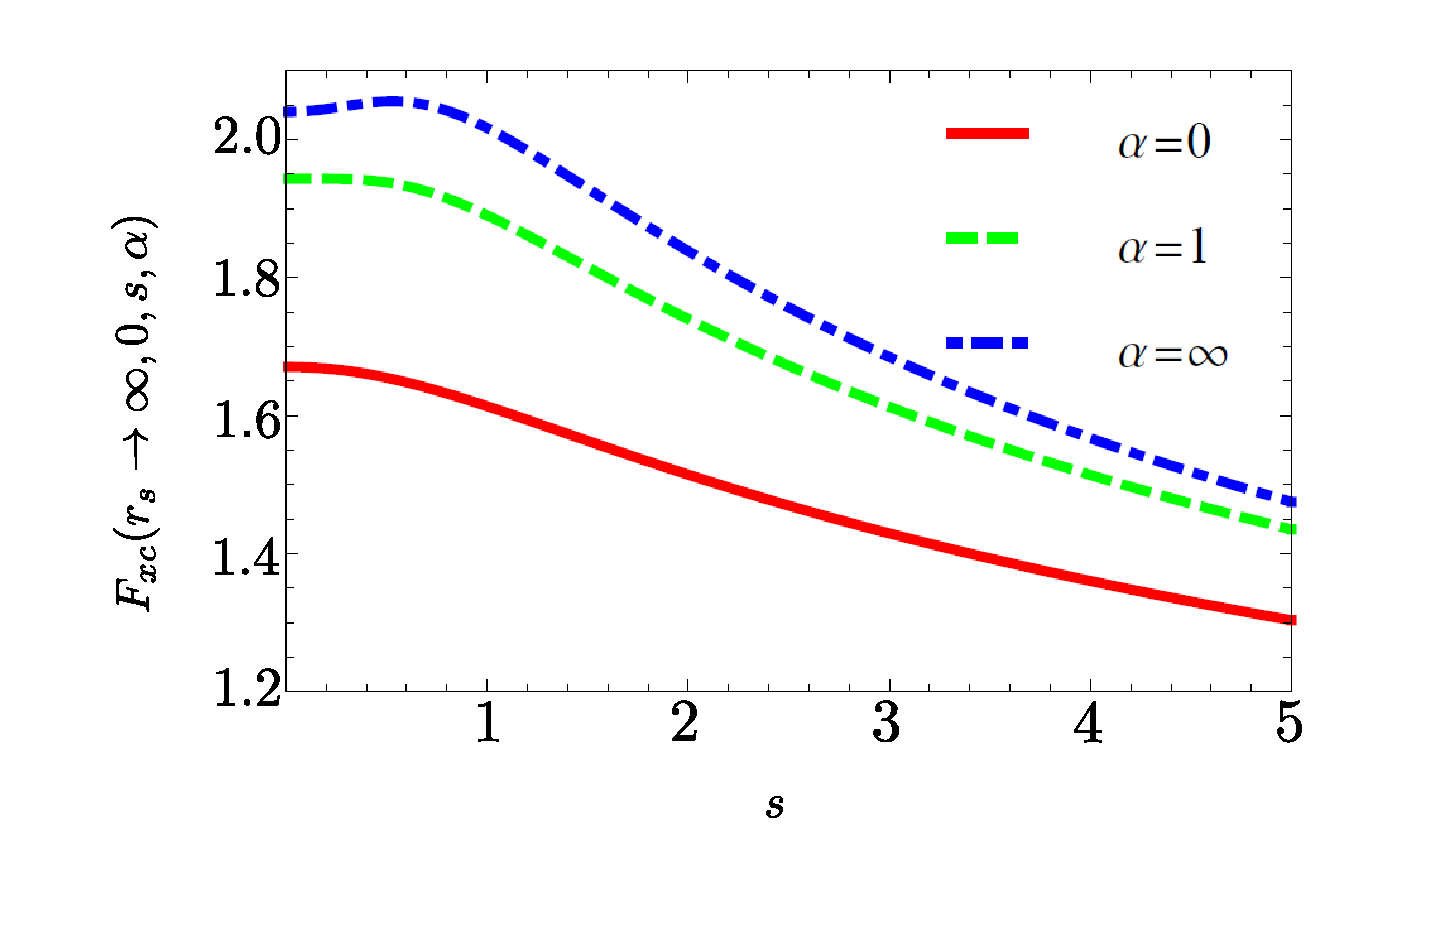
\includegraphics[width=1.0\linewidth]{F_factor1v3.pdf}
    	\caption{Фактор посилення обмінної кореляції в межі низької густини для спін-неполяризованого випадку.}
    	\label{fig:sub1}	
	\end{subfigure}
	
	\begin{subfigure}{.9\textwidth}
		\hspace*{0.15cm}
    	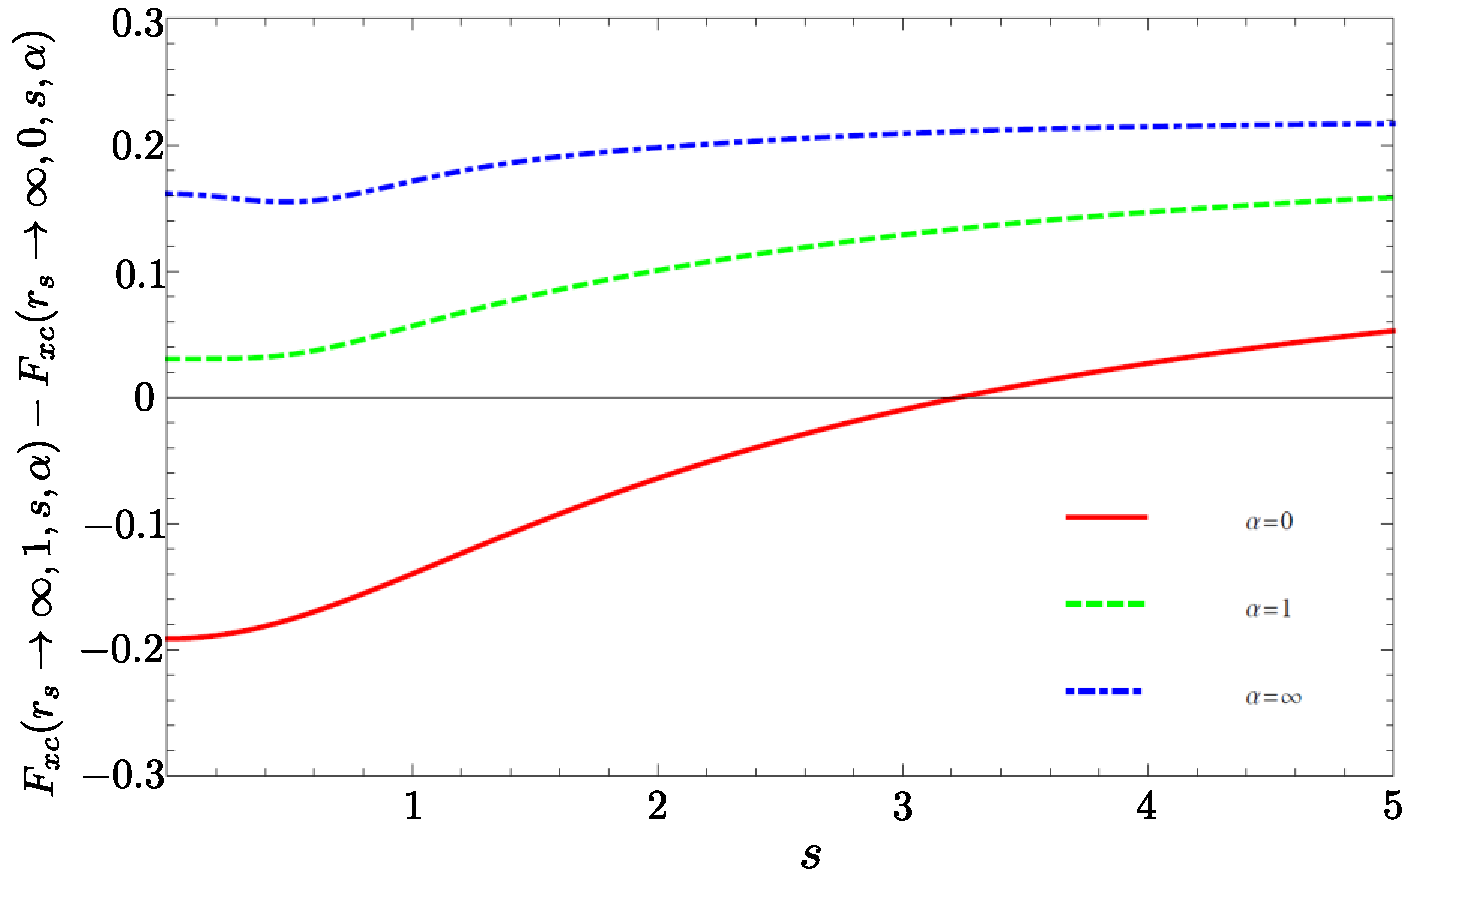
\includegraphics[width=1.0\linewidth]{F_factor2.pdf}
    	\caption{
    	Різниця між повністю спін-поляризованим ($\xi = 1$) і неполяризованим ($\xi = 0$) фактором посилення обмінної кореляції в межі низьких густин ($r_s \rightarrow \infty$).}
    	\label{fig:sub1}	
	\end{subfigure}
\caption{Фактор посилення при низькій щільності градієнту.}
\end{figure}

\section{Взаємодія Хаббарда: DFT + U}
Багато з найцікавіших проблем фізики конденсованих середовищ пов'язані з матеріалами, в яких електрони мають тенденцію локалізуватися і сильно взаємодіяти, такими як оксиди перехідних металів і рідкісноземельні елементи, а також сполуки, які частково займають $d$ і $f$ стану. Звичайні функціонали, такі як LDA і GGA, виявляють, що система являє собою метал, але насправді це магнітний ізолятор. Навіть якщо енергія основного стану визначена правильно, то зонні спектри сильно можуть відрізнятися від того, що ми бачимо в експерименті. Фундаментальна проблема полягає у тому що не існує унікального шляху для визначення локальних орбіталей. 

Абревіатура "LDA+U" часто використовується для позначення методів, які включають обчислення типу LDA або GGA в поєднанні з додатковою орбітально-залежною взаємодією \cite{PhysRevB.44, Anisimov1997}, але в цій роботі використовується більш загальний термін "DFT+U." додаткова взаємодія зазвичай розглядається тільки для високолокалізованих атомно-подібних взаємодій, орбіталі на тій же ділянці, тобто тієї ж форми, що і взаємодія "U" в моделях Хаббарда. Ефект доданого члена полягає в зміщенні локалізованих орбіталей відносно інших орбіталей, що намагається виправити помилки, які, як відомо, є великими в звичайних обчисленнях LDA або GGA. Наприклад, енергії просування в атомах перехідних металів ілюструють той факт, що відносні енергії зміщуються в залежності від наближення для обміну. Інший ефект виникає в частково заповнених $d$ і $f$ станах, де заняття однієї орбіталі підвищує енергію інших орбіталей, в результаті чого це сприяє магнітним станам. Оскільки ефекти мають вирішальне значення для багатьох завдань, пов'язаних з $3d$ оксидами перехідних металів та іншими матеріалами, розрахунки "DFT+U" є невід'ємною частиною сучасних методів.

Багато прикладів обчислень "DFT+U" наведені в \cite{Anisimov1997}. Прототипними прикладами є оксиди перехідних металів. Можливо, найбільш відомими прикладами є вихідні сполуки надпровідників CuO, які, як виявилося, є немагнітними металами в звичайних розрахунках LDA і GGA, тоді як розрахунки "DFT+U" знаходять правильне рішення для антиферомагнітного ізолятора \cite{Anisimov1997}. Звичайна теорія спінової щільності для таких матеріалів, як MnO та NiO, знаходить правильні спінові стани і енергетичну щілину, але величина щілини занадто мала, як показано на рис. \ref{fig:GAP}. Розрив набагато краще з гібридними функціоналами; однак часто простіше і інтуїтивно зрозуміліше виправити розрив за допомогою члена "U", який збільшує розрив між заповненим і порожнім $3d$-станами і здвигає стани до станів кисню, щоб вони набагато краще узгоджувалися з експериментом.

\begin{figure}[H]
	\centering
	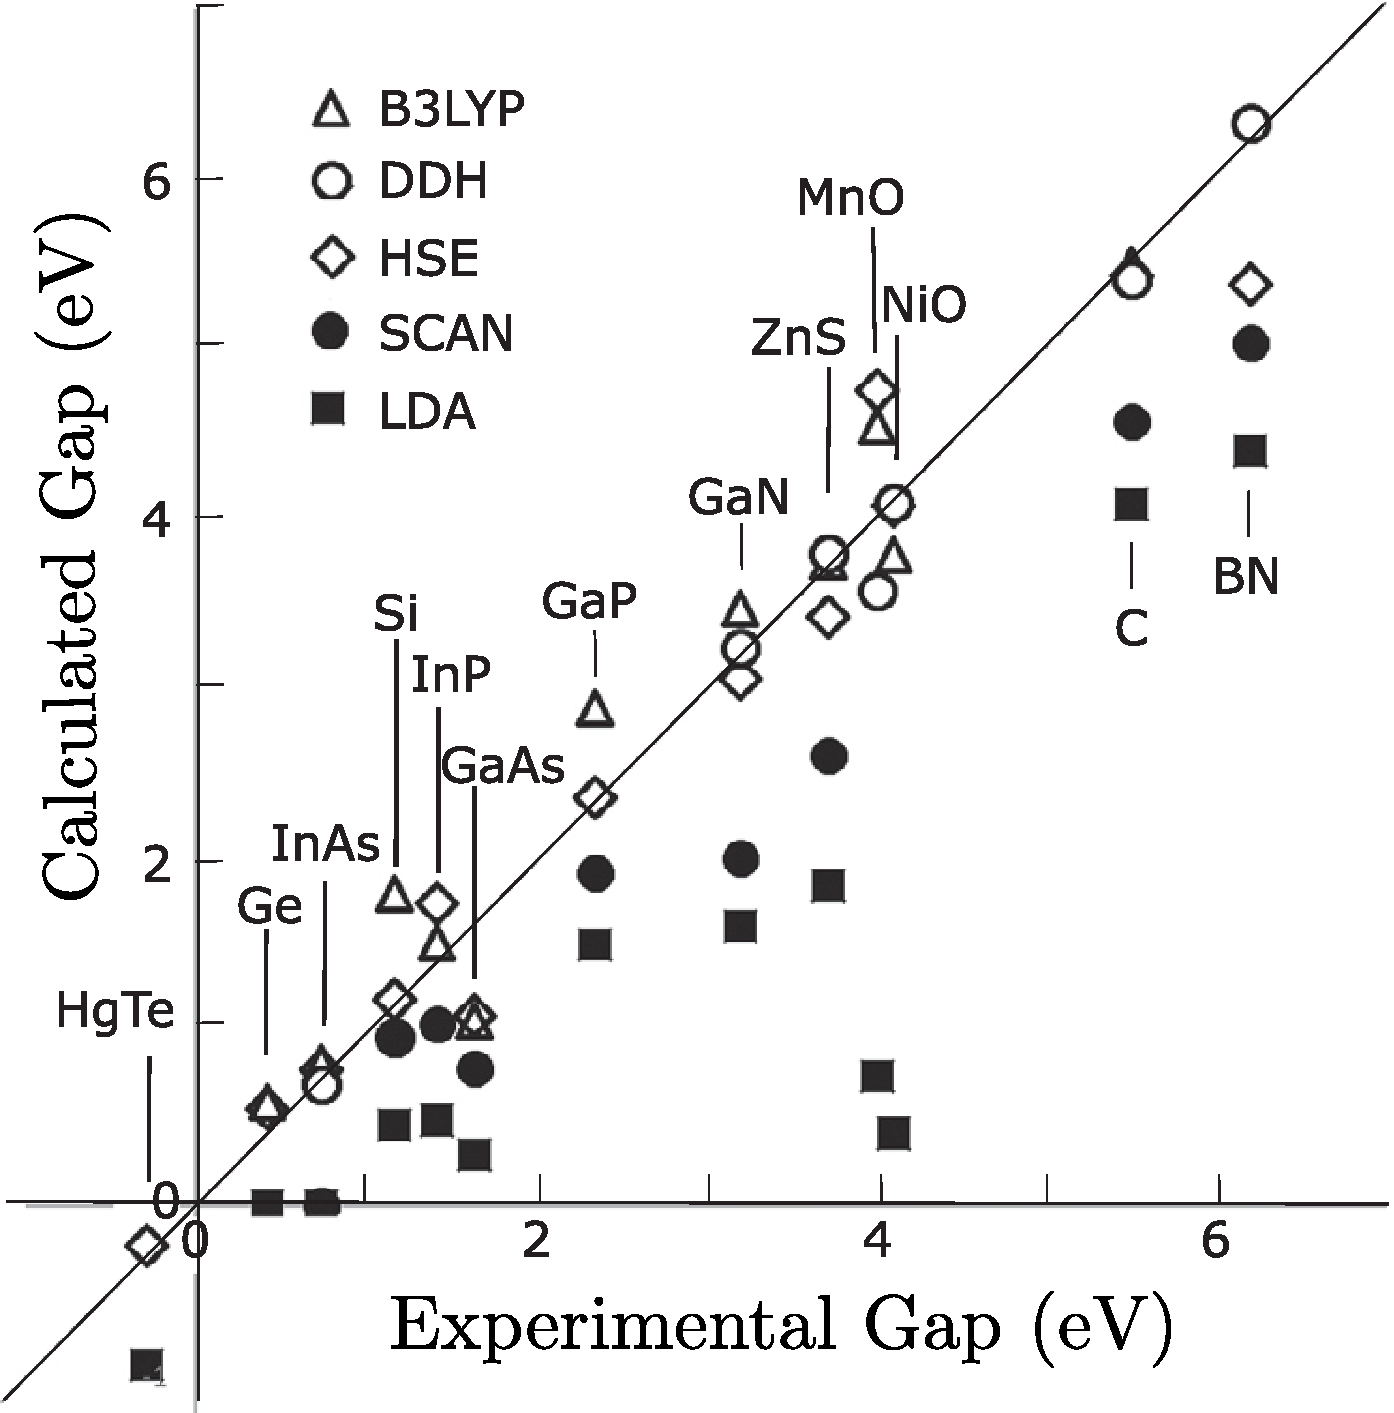
\includegraphics[scale=0.5]{GAP.pdf}
	\caption{Заборонені зони в порівнянні з експериментом для різних функціоналів. Функціонали LDA і meta-GGA позначаються закритими символами, а гібридні функціонали - відкритими символами. В цілому, гібридні функціонали набагато краще підходять для прогалин, але вони вимагають значно більших обчислювальних зусиль.}
	\label{fig:GAP}
\end{figure}

\section{Висновки до розділу}
У даному розділі був зроблен короткий вступ до Теорії Функціоналу Густини та огляд існуючих апроксимацій обміно-кореляційного потенціалу $E_{xc}$ (поза обговоренням залишись гібридні функціонали).
Енергія основного стану, електронна щільність і пов'язані з ними властивості звичайної матерії можуть бути ефективно обчислені, коли обмінно-кореляційна енергія як функціонал щільності апроксимується напівлокально. В даній роботі запропоновано мета-GGA (мета-узагальнену градієнтну апроксимацію), яка повністю обмежена, підкоряючись всім 17 відомим точним обмеженням. Він також точний або майже точний для набору відповідних норм, включаючи атоми рідкісних газів і незв'язані взаємодії. SCAN meta-GGA забезпечує чудову точність для систем, в яких точна обмінно-кореляційна дірка локалізована поблизу її електрона, і особливо для постійних решітки і слабких взаємодій.

Для описання досліджуваних систем був обраний SCAN функціонал з додаванням Хаббардовської взаємодії. З тих причин, що SCAN не достатньо все ж таки точний, щоб описувати сильнокорельовані системи.




